\appendix

%%%%%%%%%% DON'T DELETE THIS, REVERTS NUMBERING BACK %%%%%%%%%%%%%
\makeatletter
\renewcommand{\@makechapterhead}[1]{\vspace *{-10\p@ }{\parindent \z@ 
\raggedright \normalfont \ifnum \c@secnumdepth >\m@ne \Huge \bfseries 
\@chapapp \space \thechapter \vskip 10\p@ \fi #1\par \nobreak \vskip 30\p@ }}
\makeatother
%%%%%%%%%% DON'T DELETE THIS, REVERTS NUMBERING BACK %%%%%%%%%%%%%

\chapter{Reciprocal Lattice and Brillouin Zone}\label{chap:BZ}
Reciprocal lattice vectors of a lattice are defined to be the wavevectors  $\va{G}$ that satisfy 
\begin{equation} \label{eq:GdotR}
    \exp(i \va{G} \vdot \va{R} ) = 1
\end{equation}
for any lattice translation vector $\va{R}$ given by
\begin{equation}
    \va{R} = n_1 \va{a}_1 + n_2 \va{a}_2 +n_3 \va{a}_3
\end{equation}
Here $n_1, n_2, n_3$ are arbitrary integers and $\va{a}_1, \va{a}_2, \va{a}_3$ are the primitive lattice vectors of the direct (real) lattice. Similarly, the reciprocal lattice vector can be resolved into its components 
\begin{equation}
    \va{G} = h \va{b}_1 + k \va{b}_2 + l \va{b}_3
\end{equation}
where $h, k, l$ are also  arbitrary integers and $\va{b}_1, \va{b}_2, \va{b}_3$ are the primitive lattice vectors of the reciprocal lattice. The integers $h, k, l$ constitute the so called Miller indices $(hkl)$. Satisfying \eqref{eq:GdotR} means that 
\begin{equation*}
    \va{a}_i \vdot \va{b}_j = 2 \pi \delta_{ij}
\end{equation*}
It can be shown that the reciprocal vectors $b_j$ can be constructed entirely in terms of real vectors $a_i$
\begin{align}
    \va{b}_1 &= 2 \pi \frac{\va{a}_2 \crossproduct \va{a}_3}{V} \\
    \va{b}_2 &= 2 \pi \frac{\va{a}_3 \crossproduct \va{a}_1}{V} \\
    \va{b}_3 &= 2 \pi \frac{\va{a}_1 \crossproduct \va{a}_2}{V} 
\end{align}
where $V = \va{a}_1 \vdot (\va{a}_2 \crossproduct \va{a}_3)$ is the volume of the unit cell. Reciprocal lattice and real lattice have important relationship. It can be shown that the reciprocal lattice vector defined by the Miller indices $(hkl)$ are perpendicular to the direct (real) lattice plane whose intercepts are the reciprocals of Miller indices $(hkl)$. 

The Brillouin Zone (BZ) is defined to be the primitive unit cell of the reciprocal lattice. The first BZ is the Wigner-Seitz cell around the wavevector $\va{k}=0$, the origin of the reciprocal space, which is defined to be the region of reciprocal space closer to $\va{k}=0$ than to any other reciprocal lattice vector. Similarly, all wavevectors that are second closest to $\va{k}=0$, constitute the second BZ, and so forth. The Wigner-Seitz cell contains only one reciprocal lattice point in it. This means that first BZ is constructed as the smallest volume entirely closed by a set of planes that are the perpendicular bisectors of the origin to each reciprocal lattice vectors. The volume of the first BZ is  related to the volume of the primitive unit cell of the real lattice
\begin{equation}
    \Omega = \frac{(2\pi)^3}{V}
\end{equation}

Brillouin zone plays a vital role in calculation of periodic systems. Owing to the periodic nature of the reciprocal lattice, any wavevectors $\va{k}$ outside the first BZ can be folded back into the first BZ by a reciprocal lattice vector $\va{G}$. In addition, any wavevectors that are shifted by a reciprocal lattice vector are all equivalent. Hence, any physical properties that have periodicity of the crystal system can be represented entirely inside the first Brillouin zone. 



















% \newpage
% \vspace*{-0.3in}
% \begin{figure}[hb!]
% \begin{center}
% \makebox[\textwidth][c]{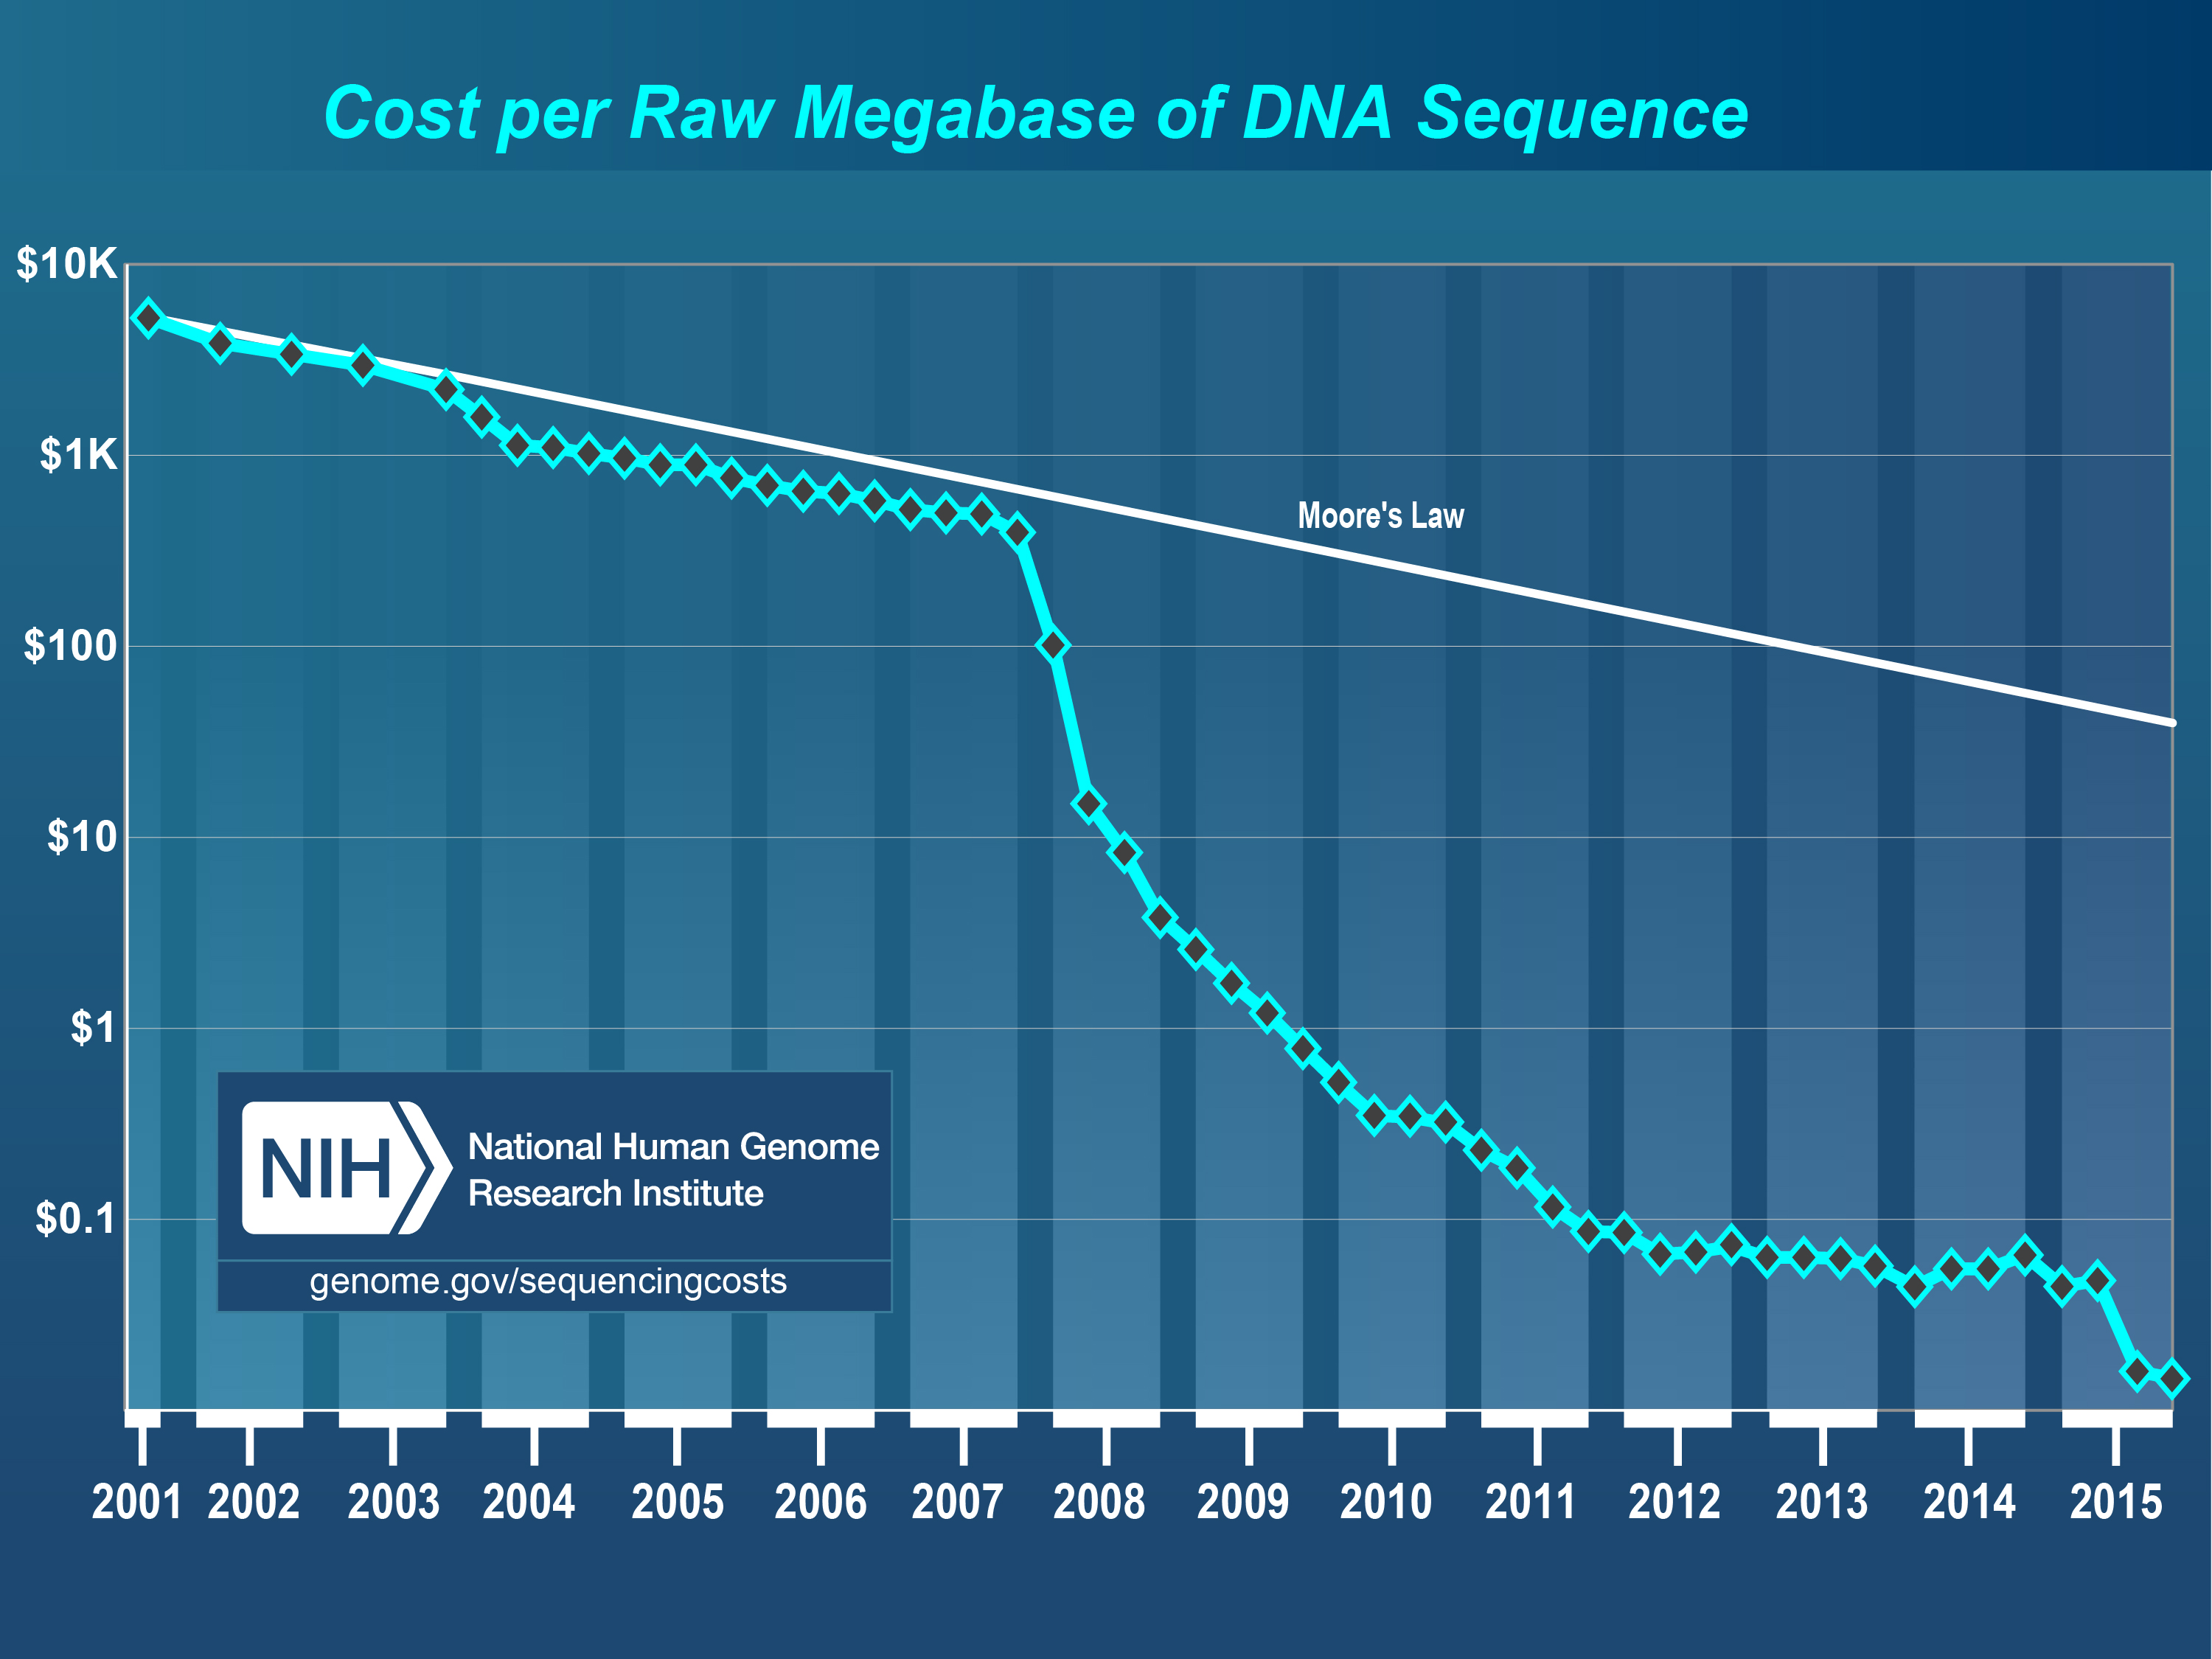
\includegraphics[width=1.0\textwidth]{costperMb2015_4.jpg}}
% \end{center}
% \caption[Cost per raw megabase of DNA sequence from 2001 to 2015]{Cost per raw megabase of DNA sequence from 2001 to 2015. Straight line - Moore's Law, blue curve - cost in US dollars, Y-axis scale is logarithmic. Graph reproduced from \citep{wetterstrand2016}}
% \end{figure}
% \begin{figure}[hb!]
% \begin{center}
% \makebox[\textwidth][c]{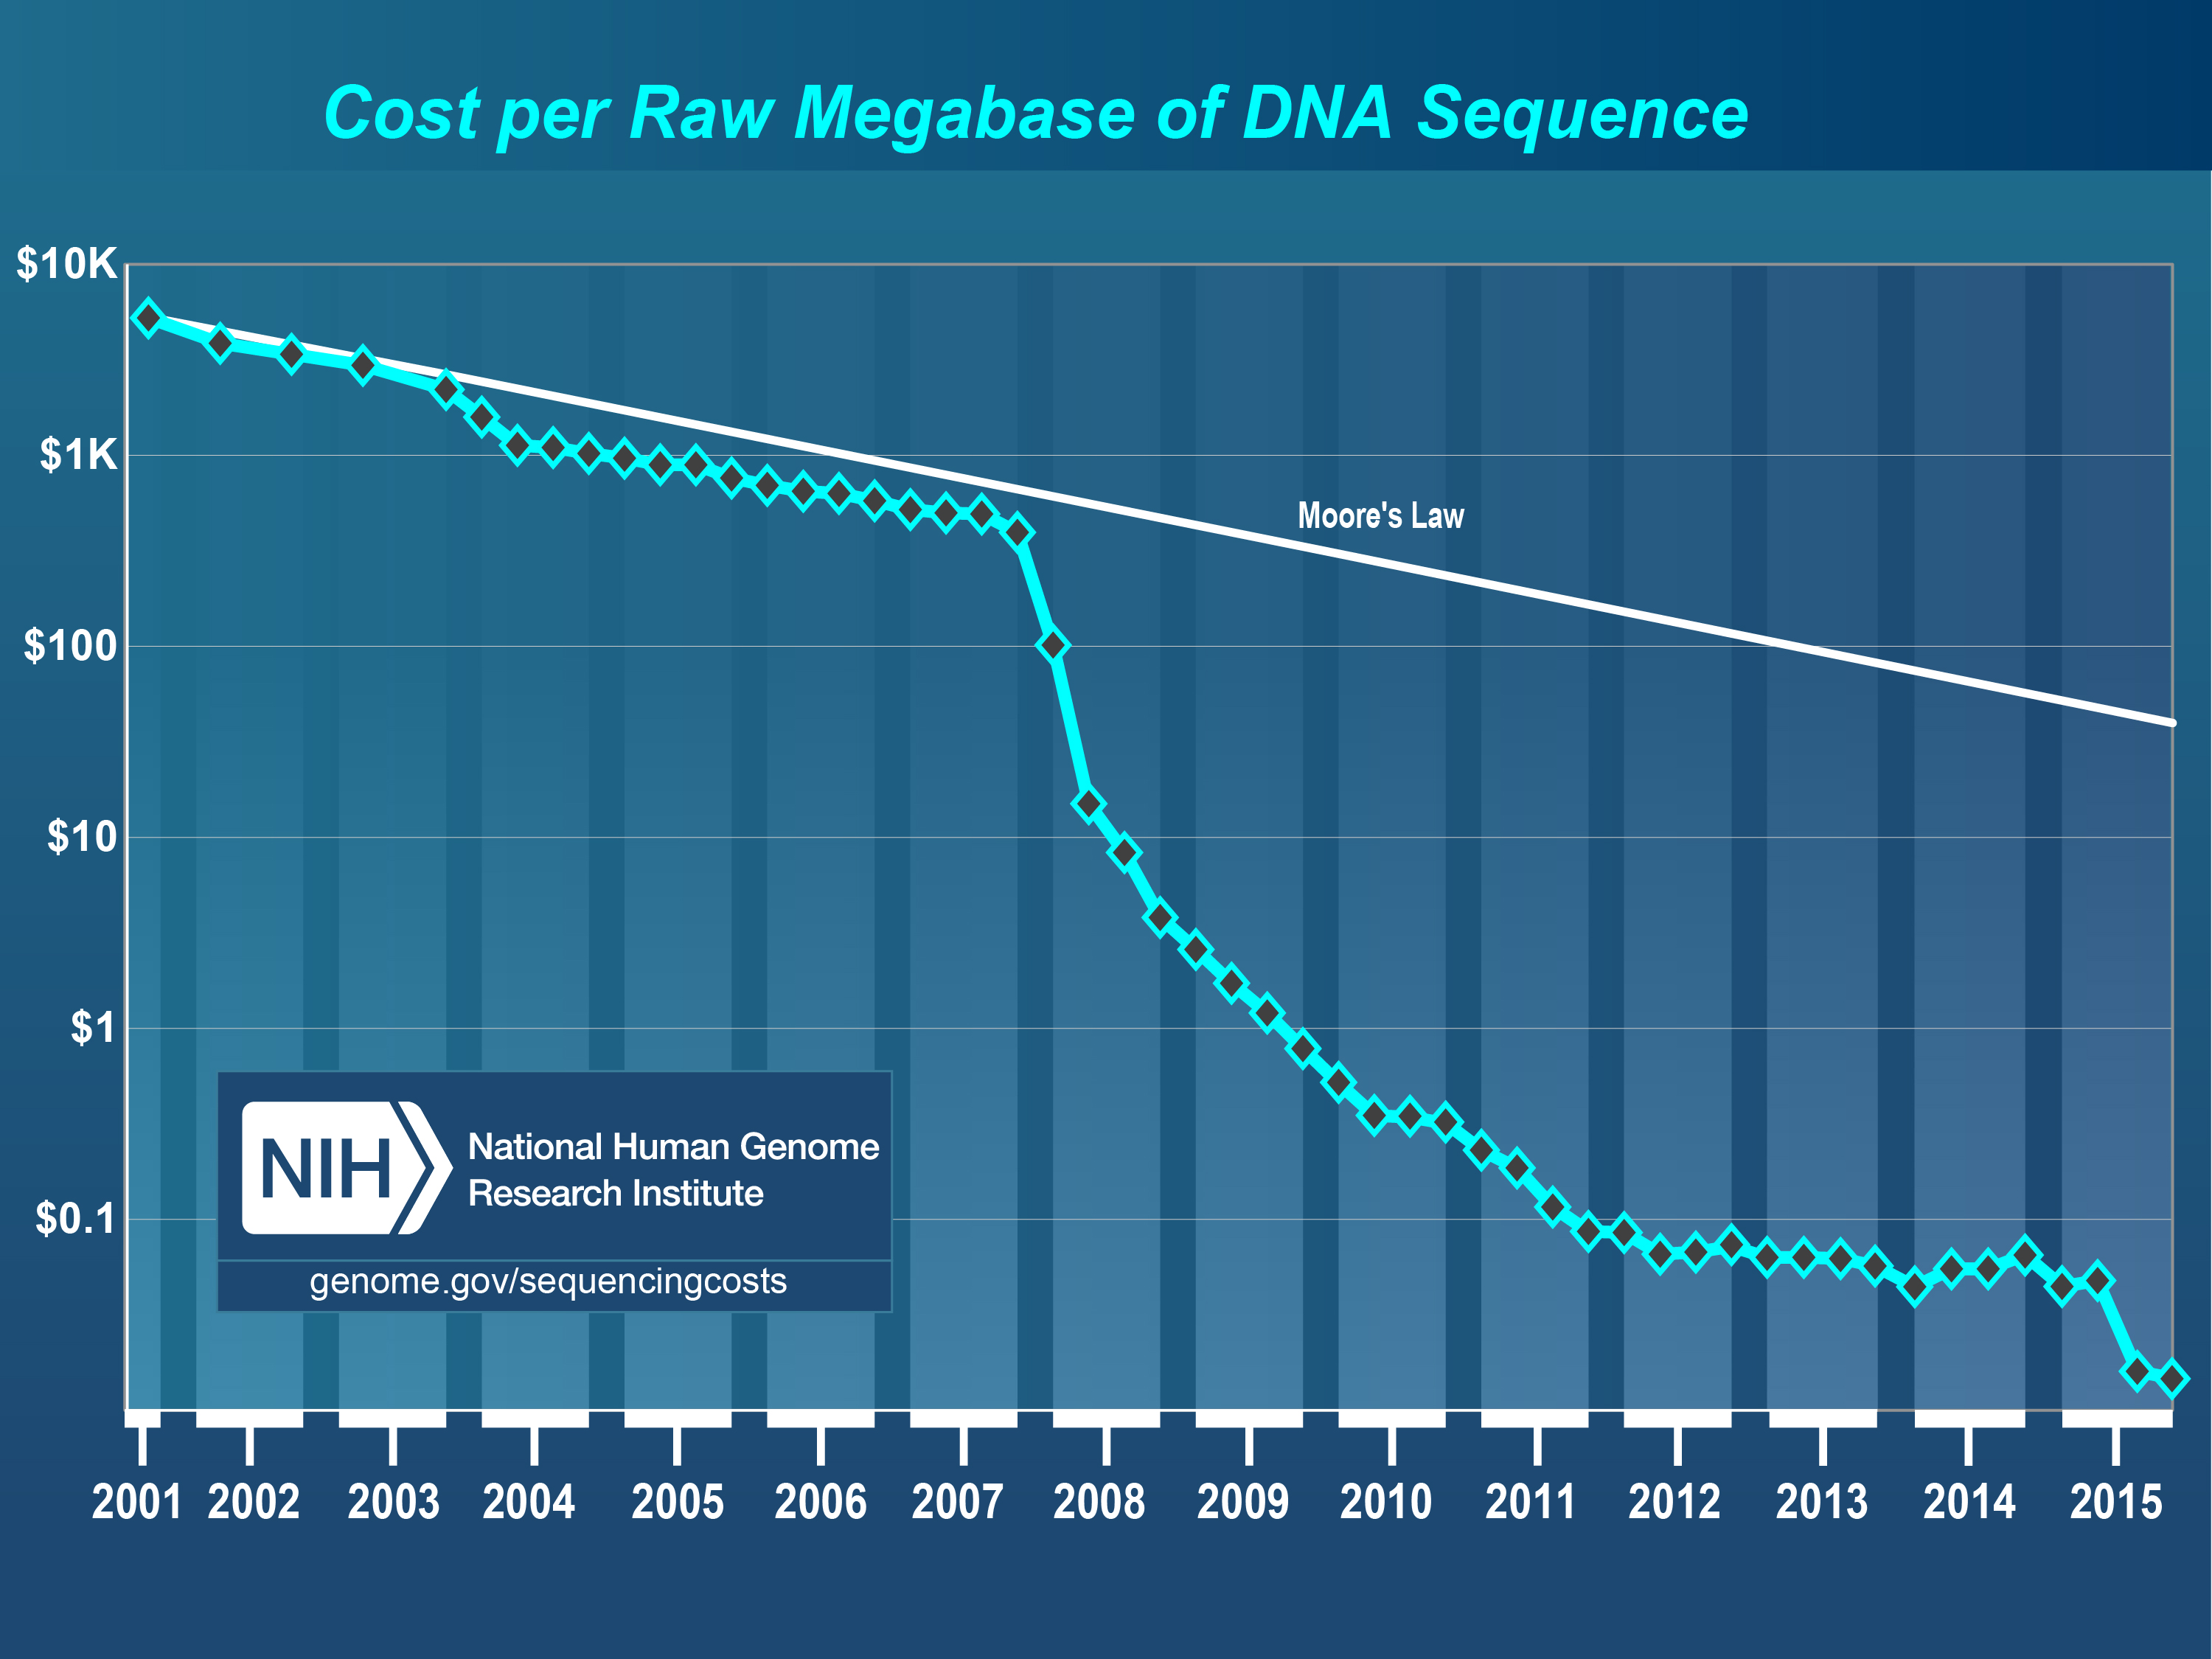
\includegraphics[width=1.0\textwidth]{costperMb2015_4.jpg}}
% \end{center}
% \caption[Cost per raw megabase of DNA sequence from 2001 to 2015]{Cost per raw megabase of DNA sequence from 2001 to 2015. Straight line - Moore's Law, blue curve - cost in US dollars, Y-axis scale is logarithmic. Graph reproduced from \citep{wetterstrand2016}}
% \end{figure}

% \chapter{}
% \vspace*{-0.3in}
% \begin{figure}[hb!]
% \begin{center}
% \makebox[\textwidth][c]{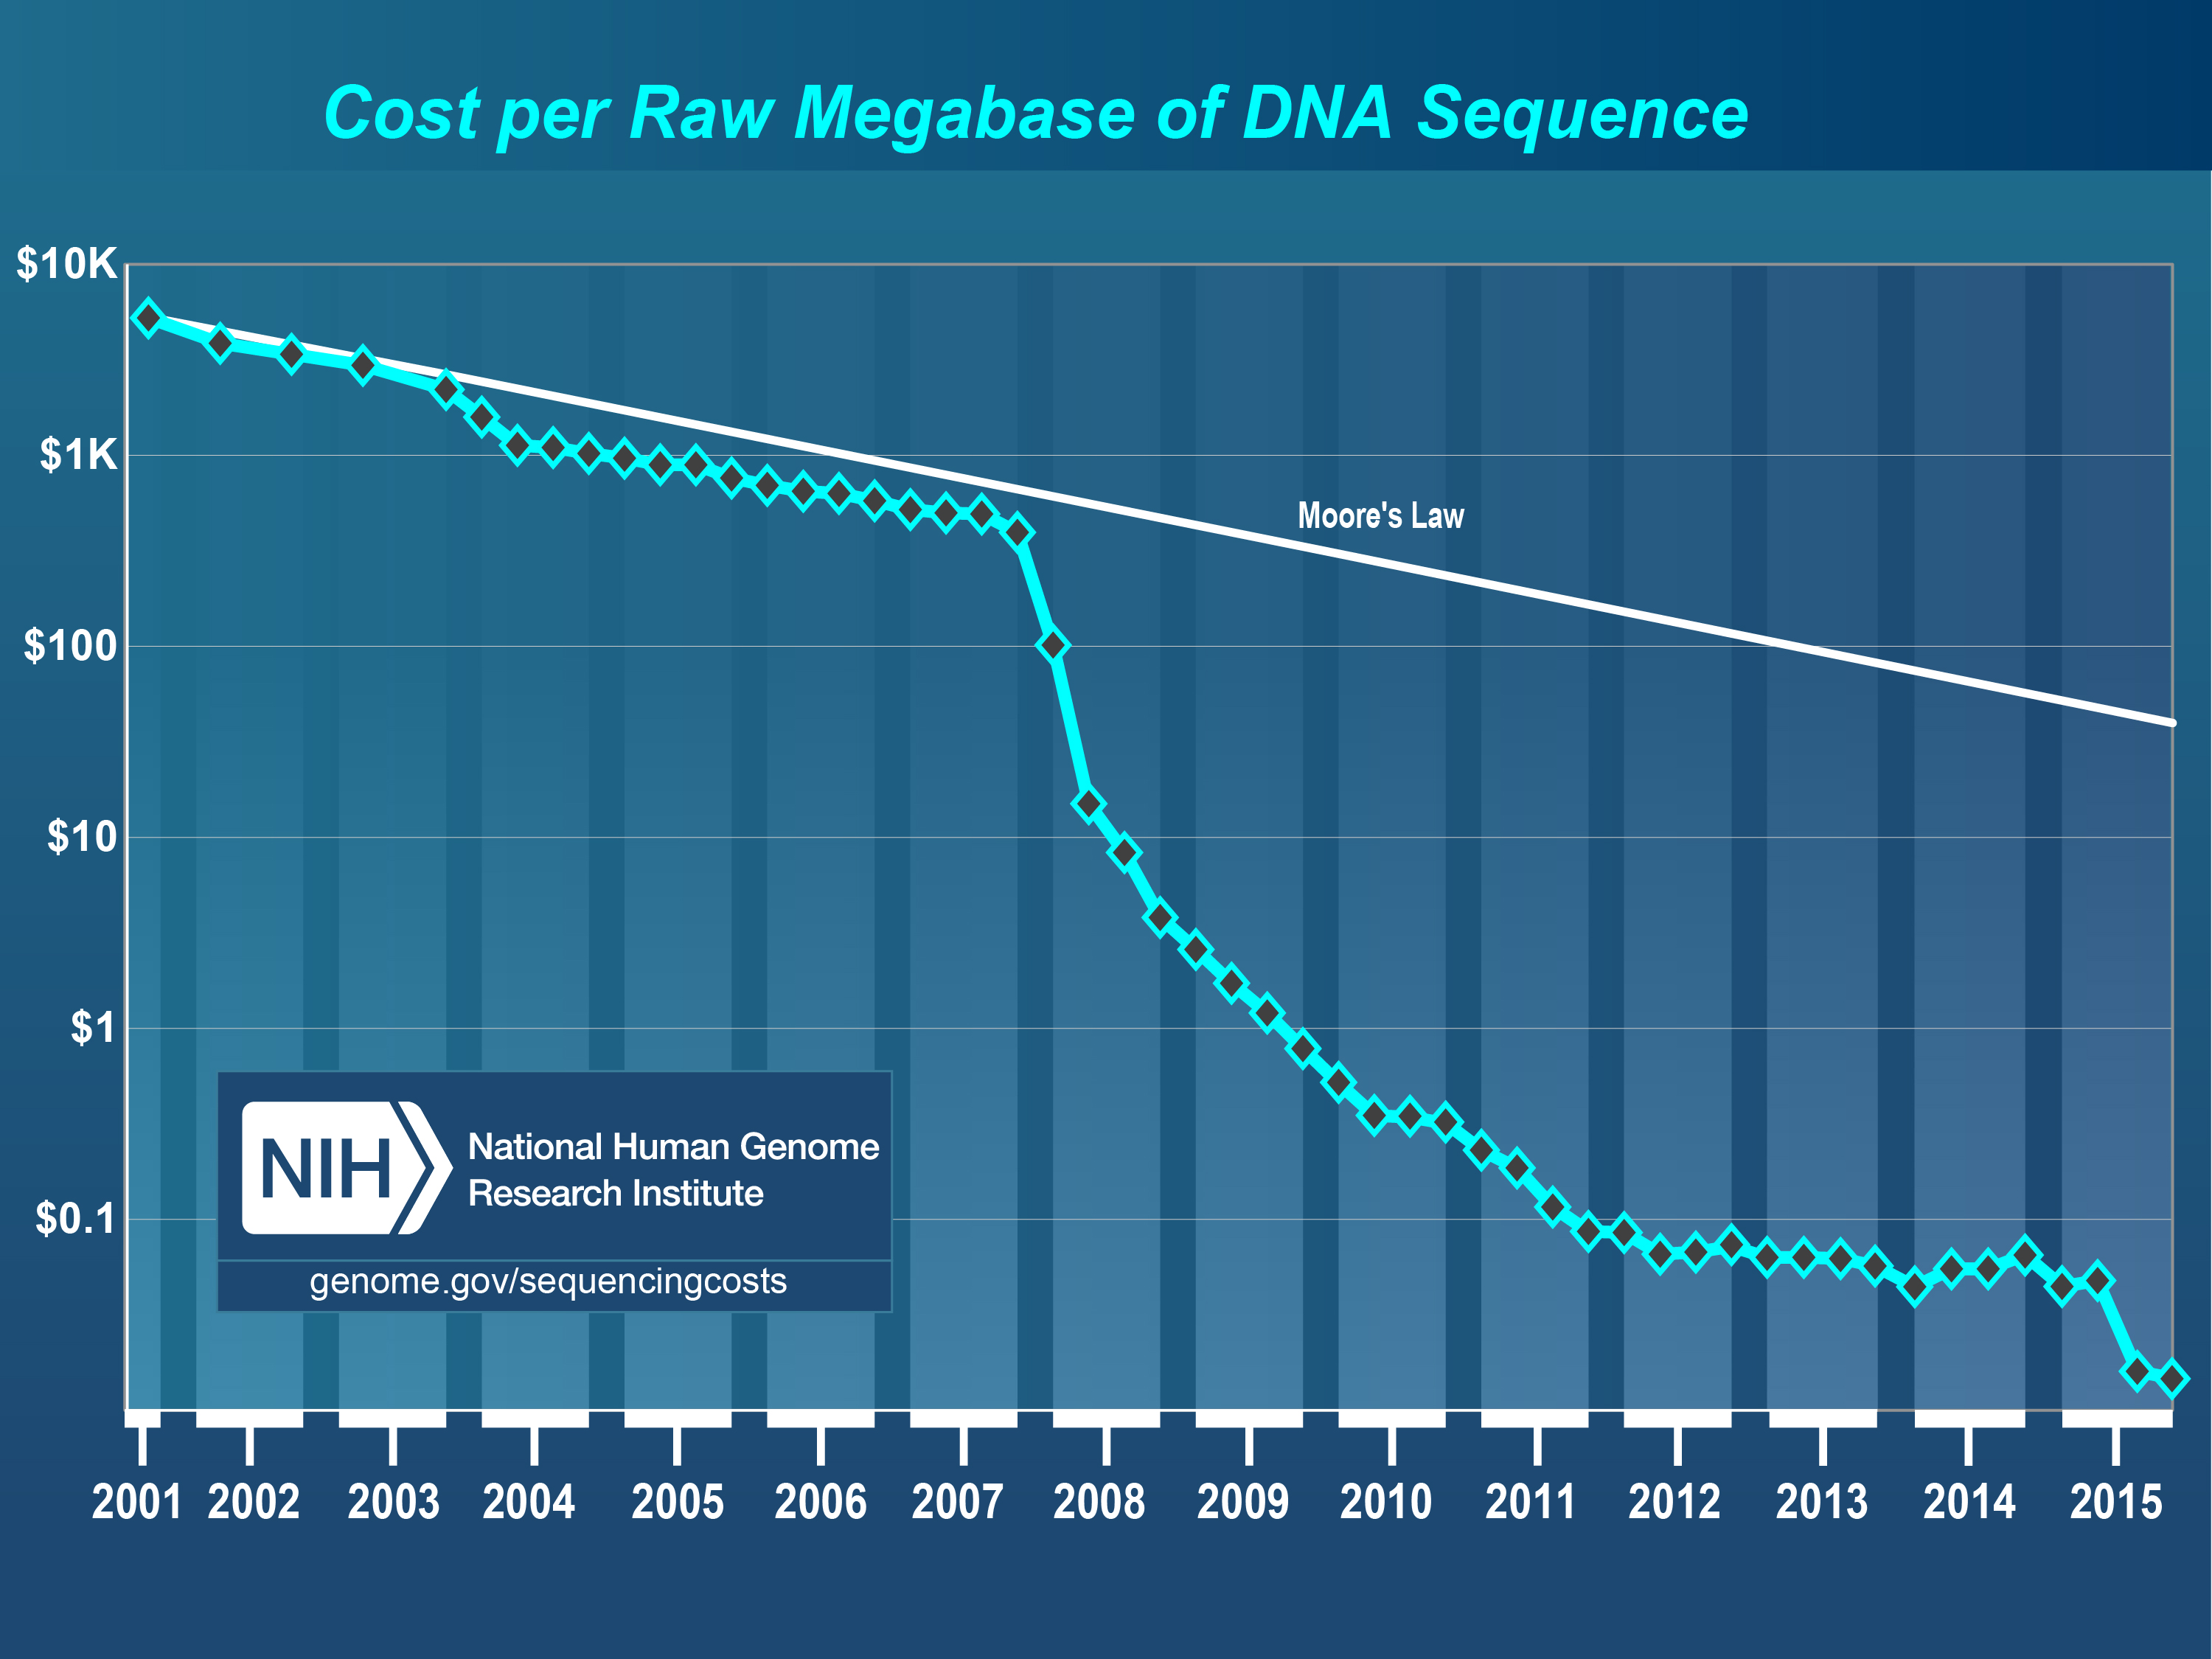
\includegraphics[width=1.0\textwidth]{costperMb2015_4.jpg}}
% \end{center}
% \caption[Cost per raw megabase of DNA sequence from 2001 to 2015]{Cost per raw megabase of DNA sequence from 2001 to 2015. Straight line - Moore's Law, blue curve - cost in US dollars, Y-axis scale is logarithmic. Graph reproduced from \citep{wetterstrand2016}}
% \end{figure}

% \chapter{}
% \begin{figure}[hb!]
% \begin{center}
% 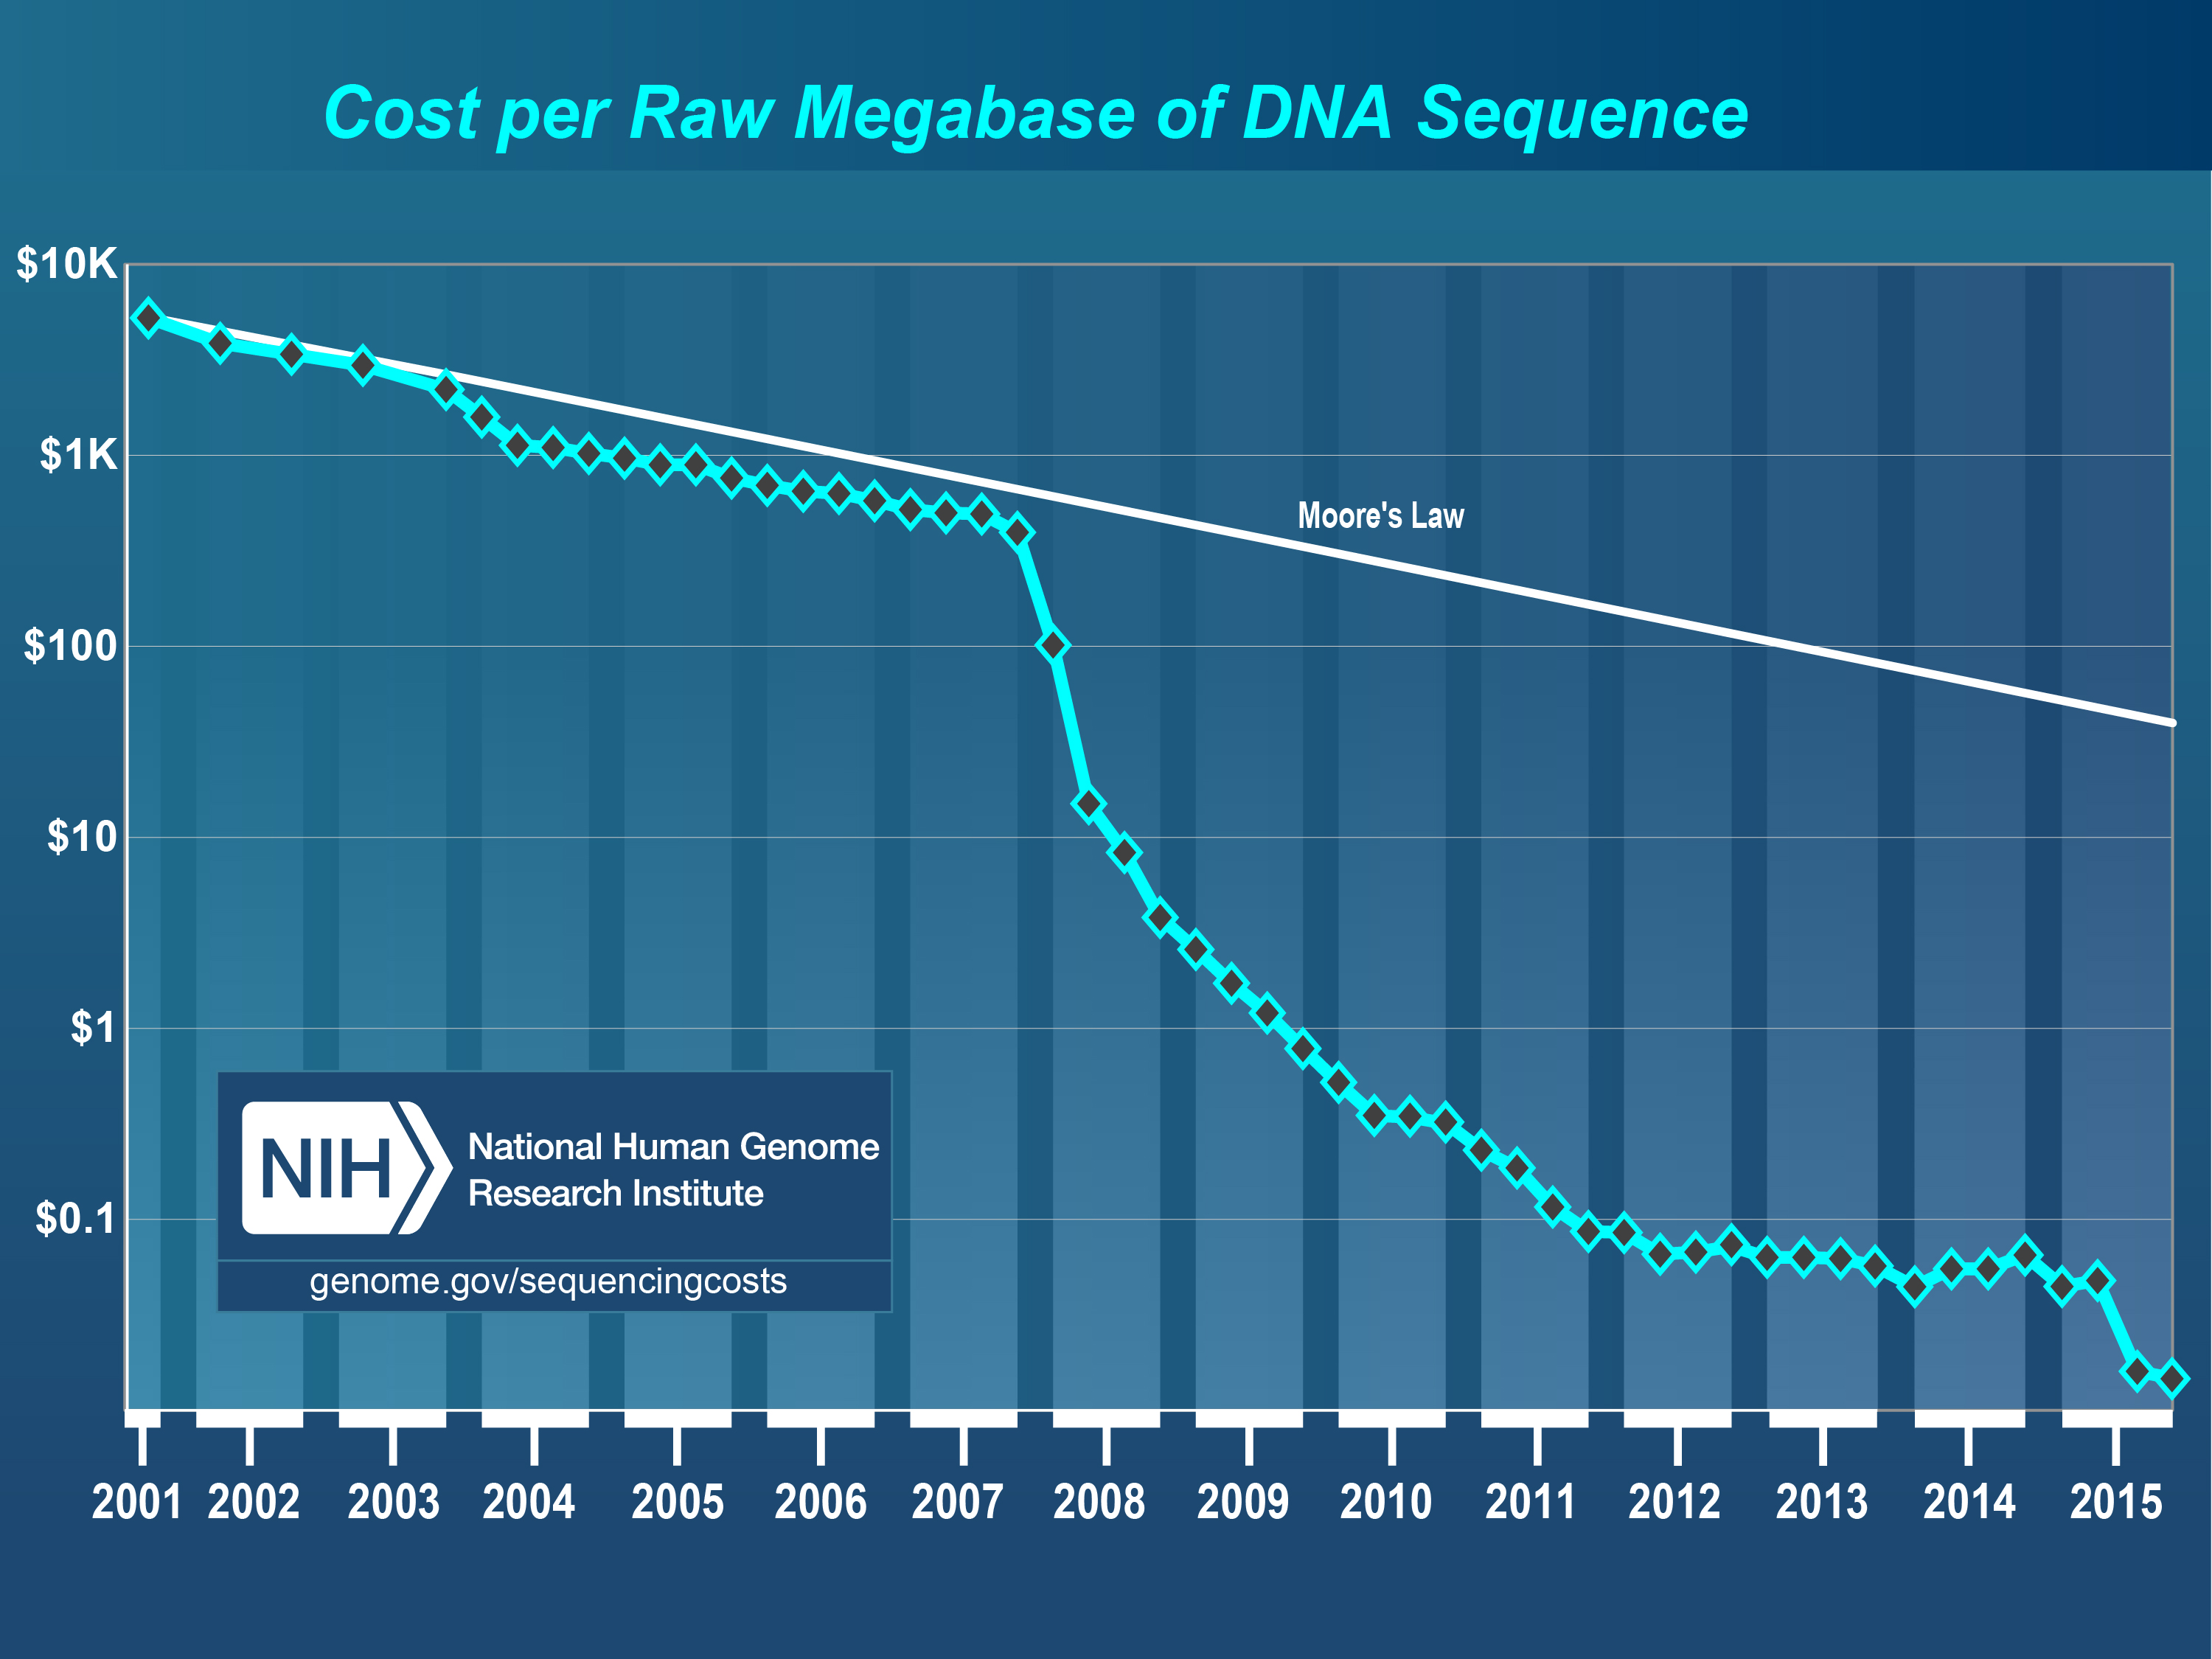
\includegraphics[scale=0.5]{costperMb2015_4.jpg}
% \end{center}
% \caption[Cost per raw megabase of DNA sequence from 2001 to 2015]{Cost per raw megabase of DNA sequence from 2001 to 2015. Straight line - Moore's Law, blue curve - cost in US dollars, Y-axis scale is logarithmic. Graph reproduced from \citep{wetterstrand2016}}
% \end{figure}

% \chapter{}
% \begin{figure}[hb!]
% \begin{center}
% 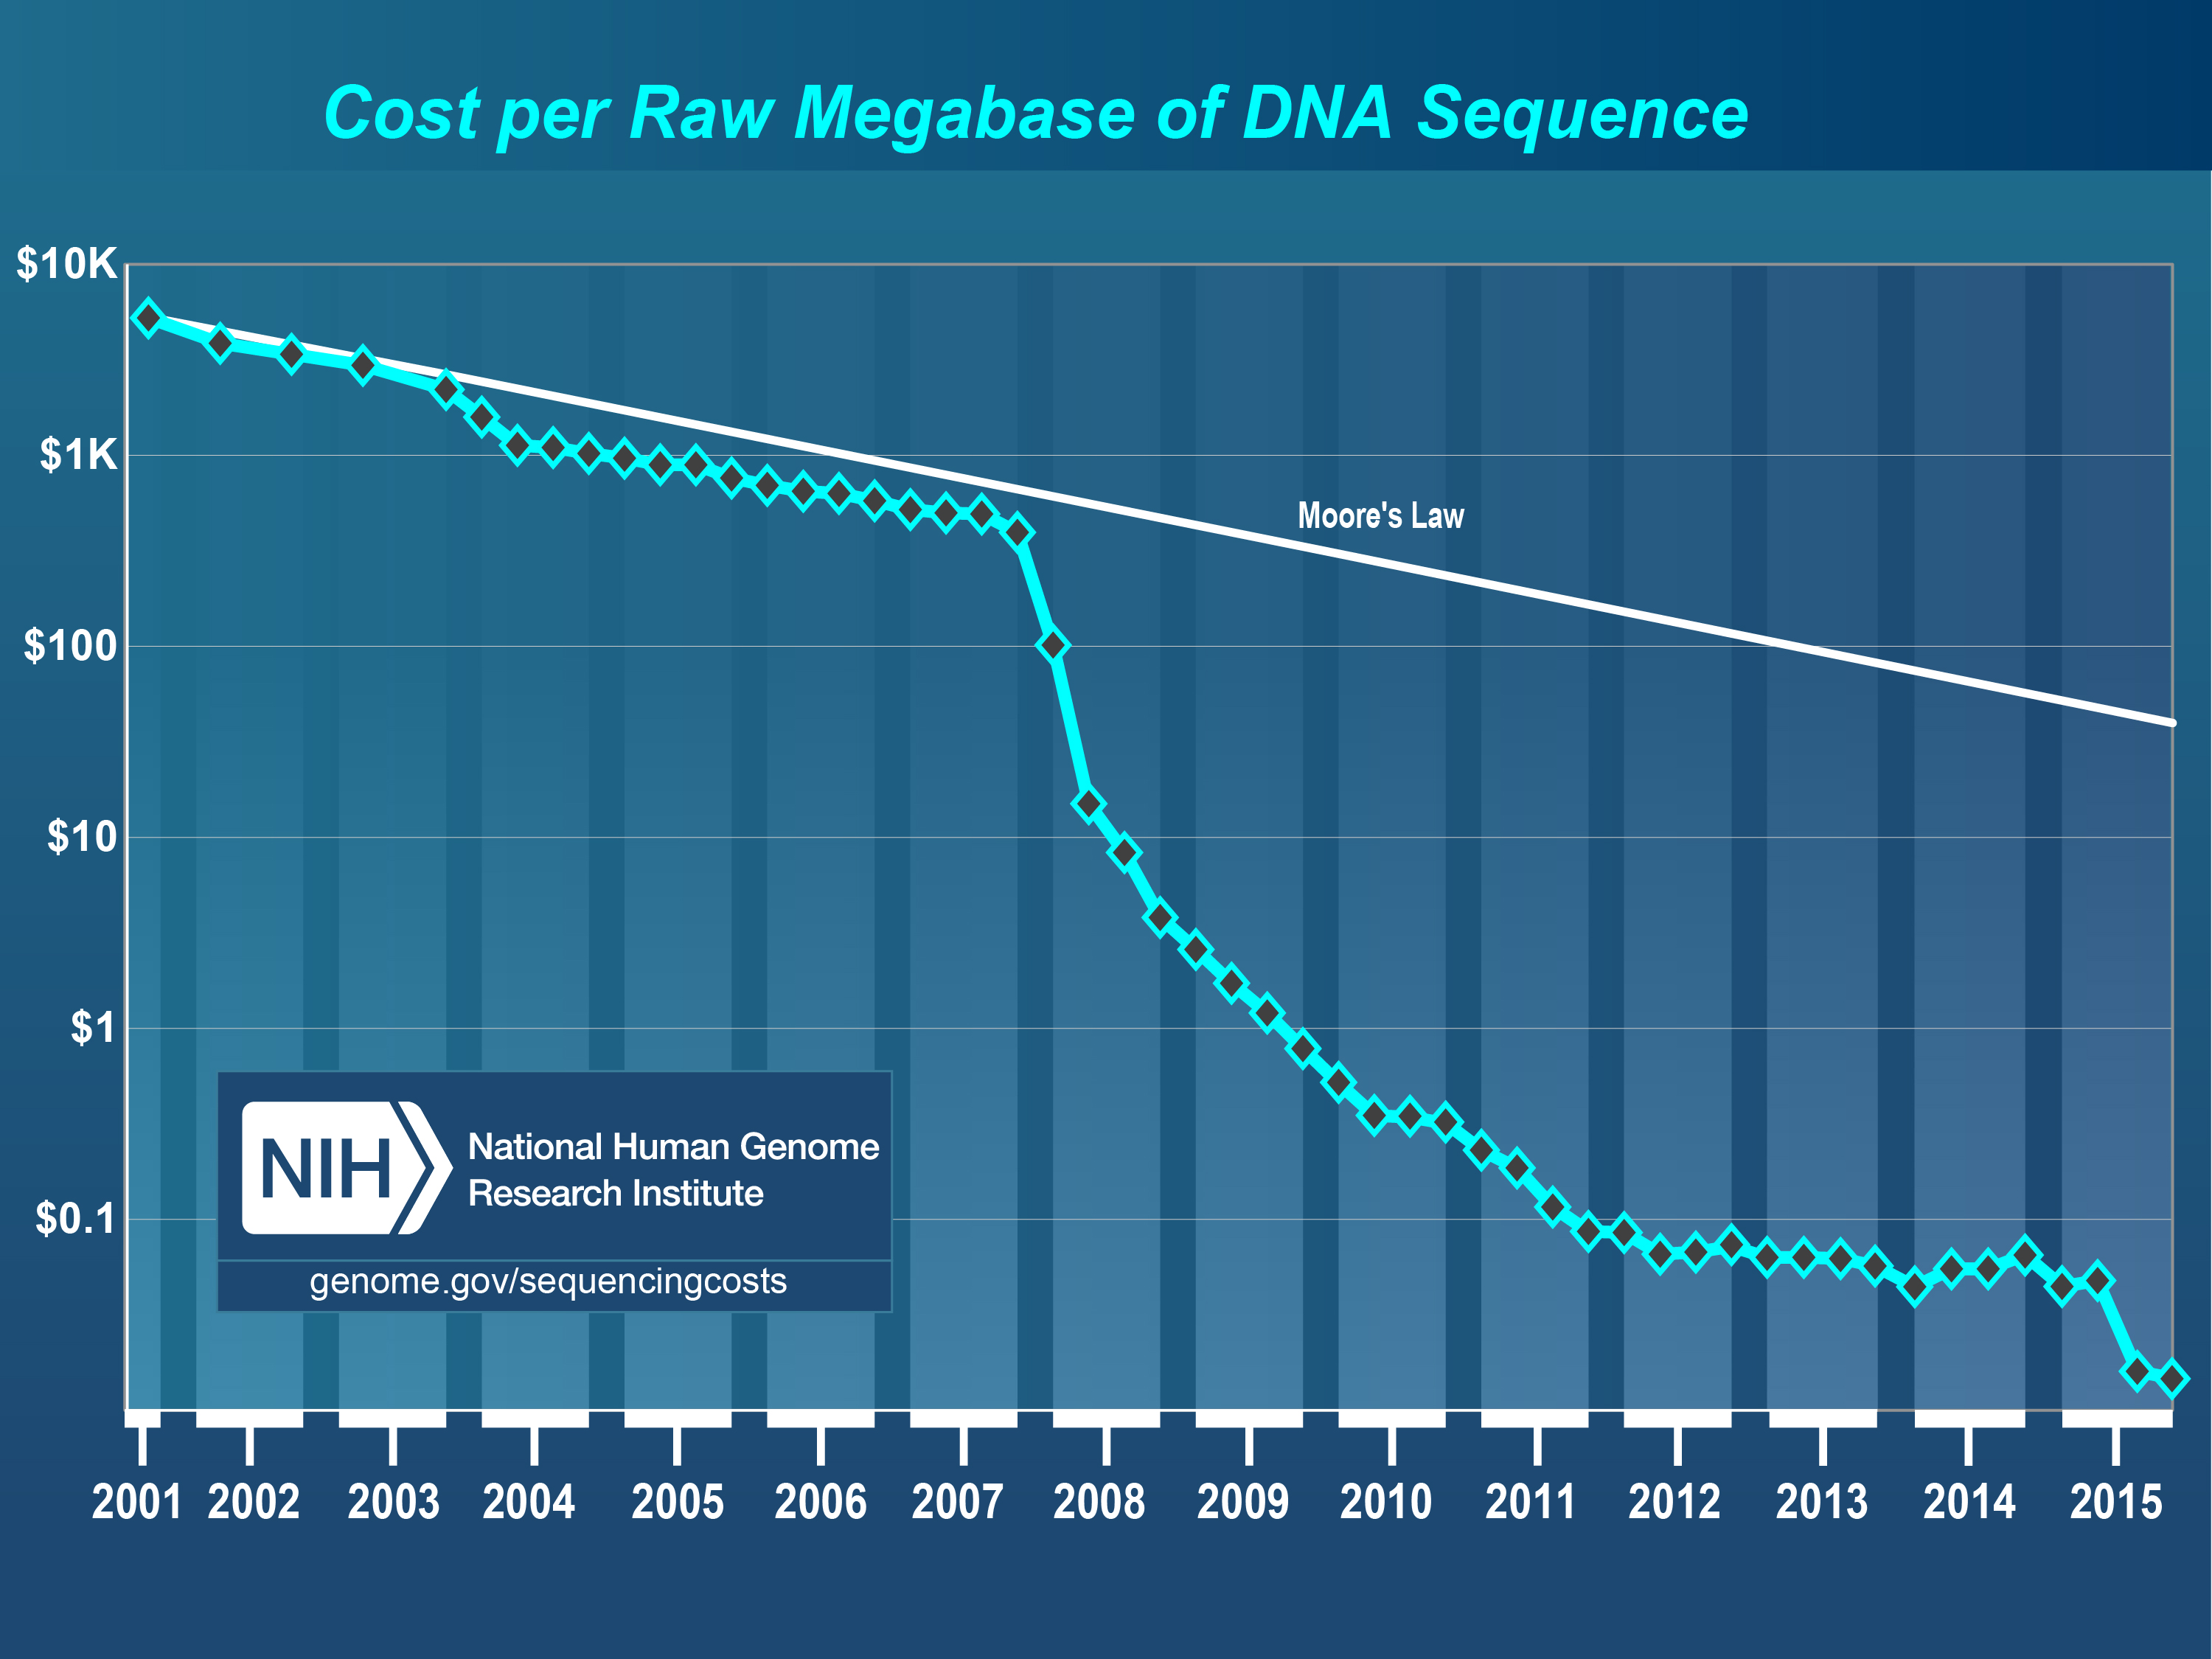
\includegraphics[scale=0.5]{costperMb2015_4.jpg}
% \end{center}
% \caption[Cost per raw megabase of DNA sequence from 2001 to 2015]{Cost per raw megabase of DNA sequence from 2001 to 2015. Straight line - Moore's Law, blue curve - cost in US dollars, Y-axis scale is logarithmic. Graph reproduced from \citep{wetterstrand2016}}
% \end{figure}

% \chapter{}
% \begin{figure}[hb!]
% \begin{center}
% 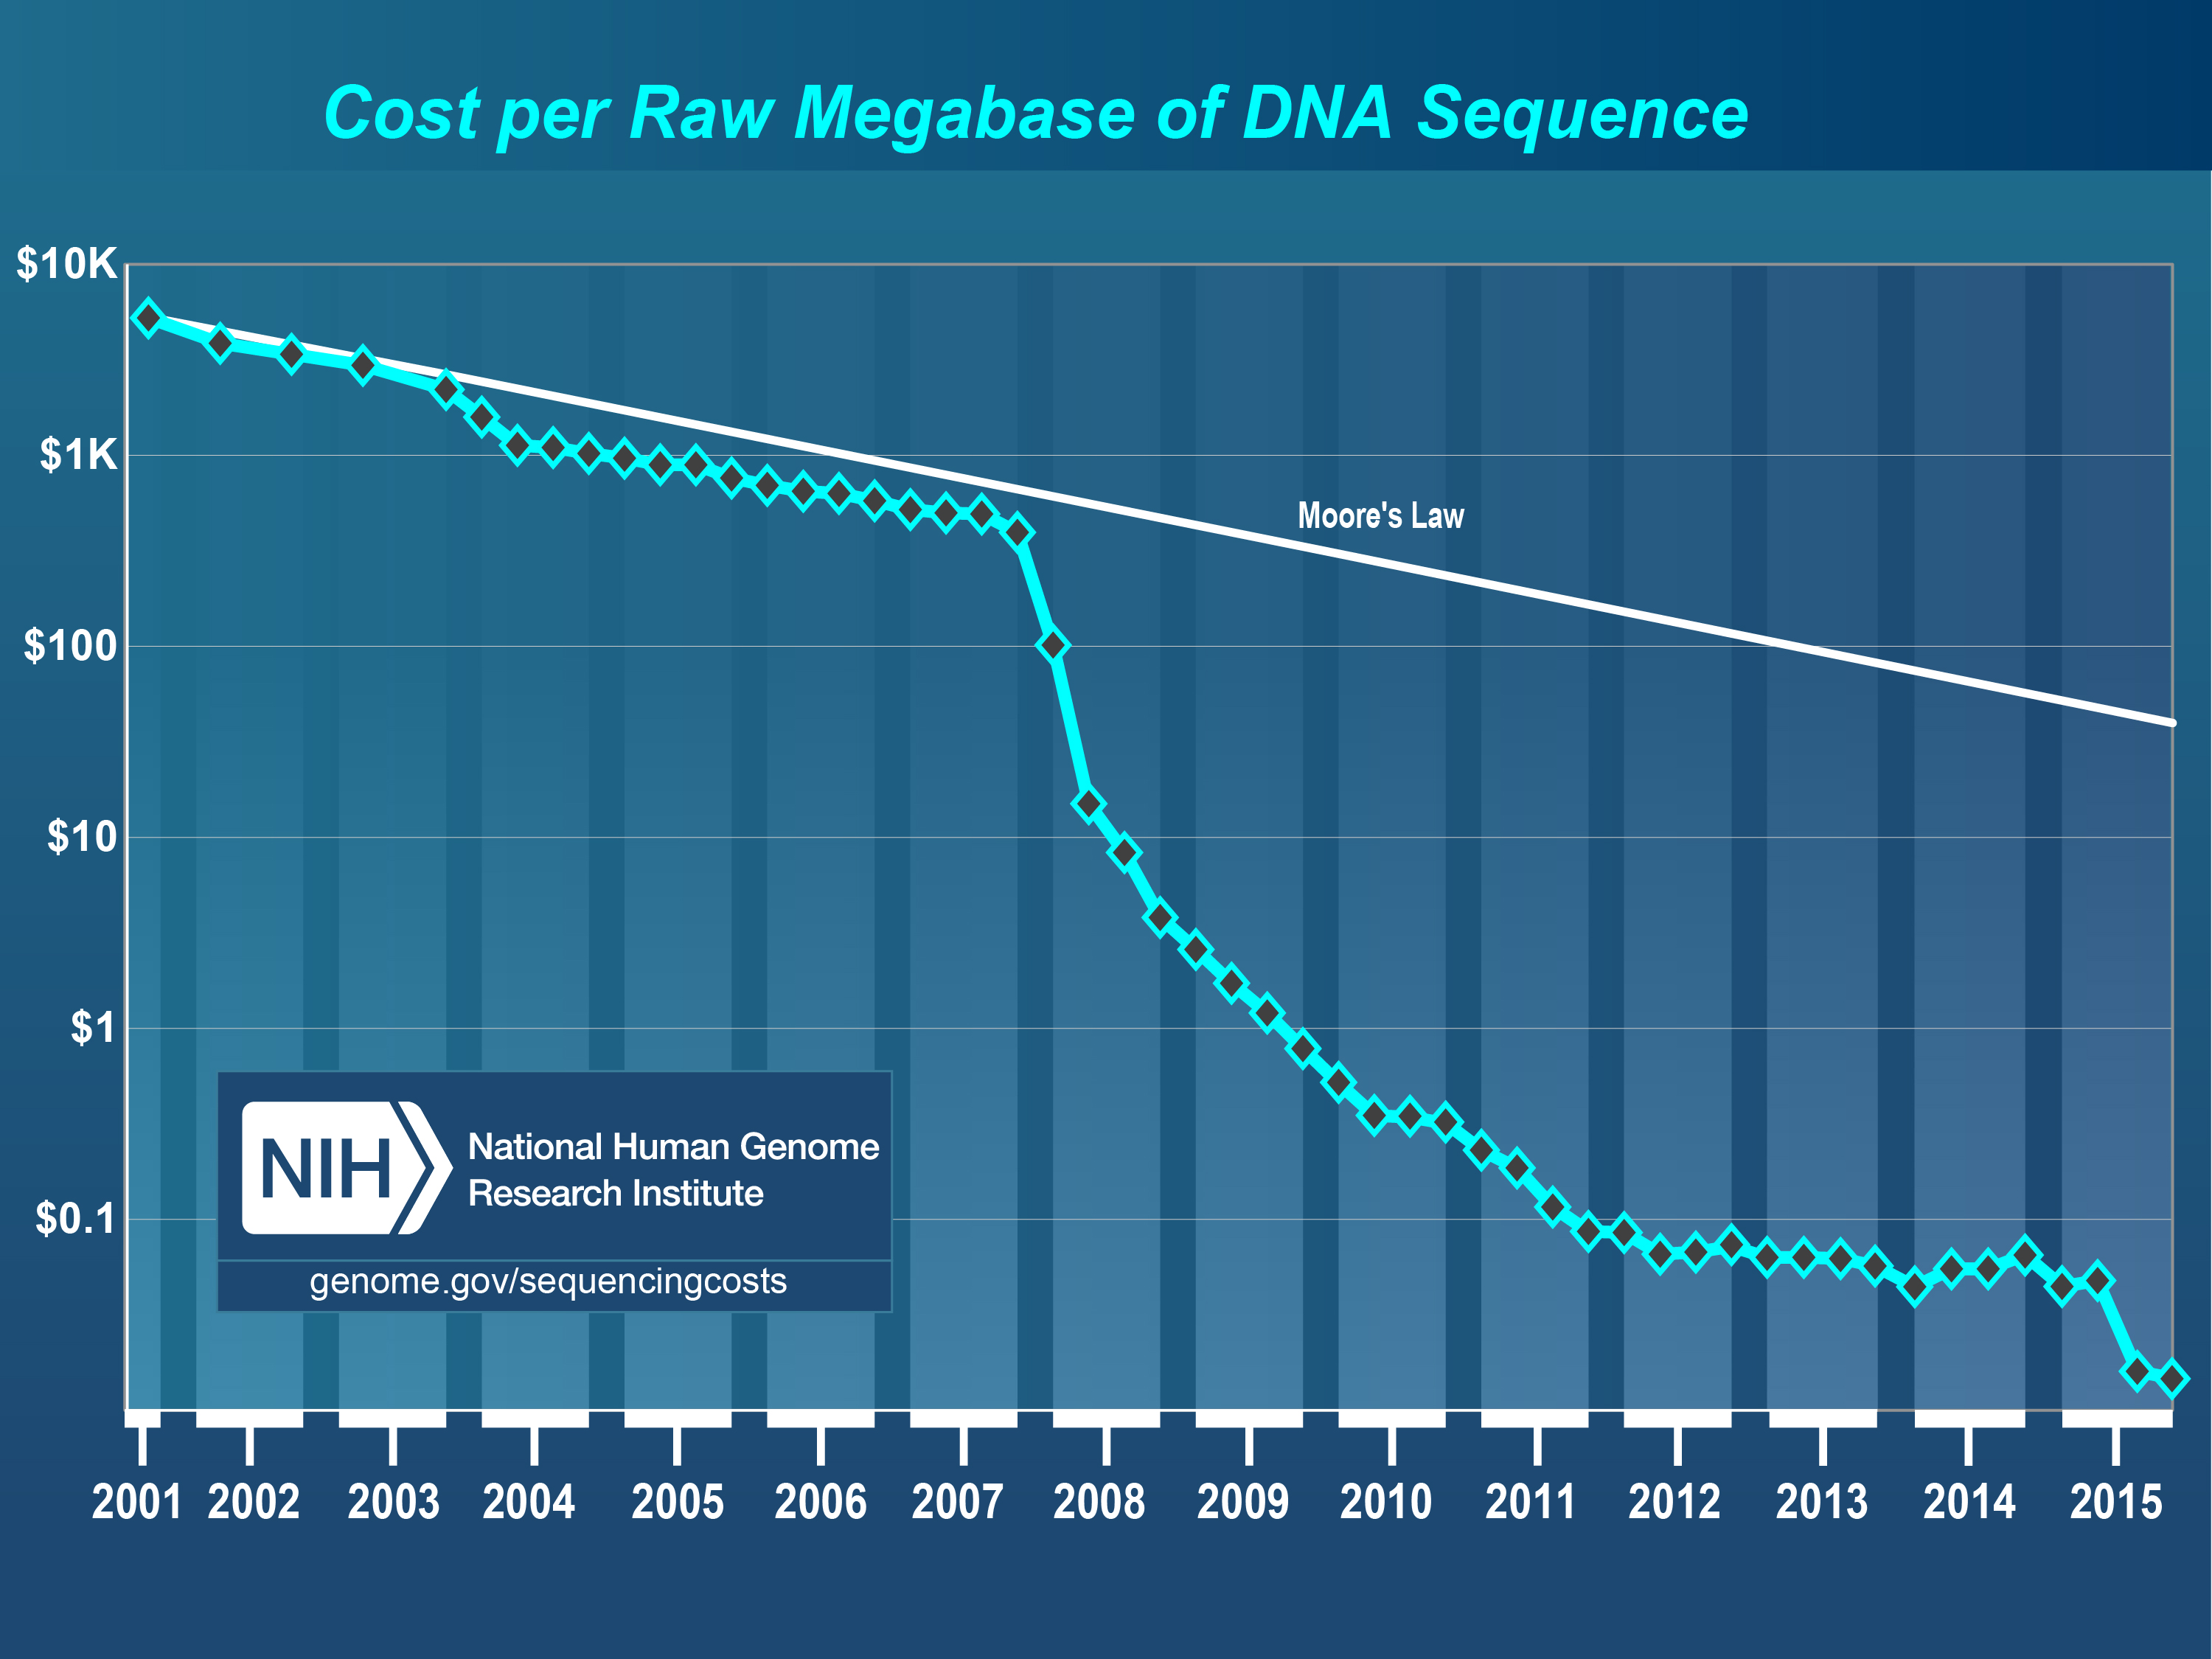
\includegraphics[scale=0.5]{costperMb2015_4.jpg}
% \end{center}
% \caption[Cost per raw megabase of DNA sequence from 2001 to 2015]{Cost per raw megabase of DNA sequence from 2001 to 2015. Straight line - Moore's Law, blue curve - cost in US dollars, Y-axis scale is logarithmic. Graph reproduced from \citep{wetterstrand2016}}
% \end{figure}

